% BTL1 slides — English version. Build PDF: tectonic slides/main-en.tex
\documentclass[aspectratio=169,11pt]{beamer}
\usepackage{amsmath,amssymb,booktabs,tikz,listings}
\usetikzlibrary{arrows.meta,positioning,calc}
% Fill in current team details before submission. Do not reuse the sample's authors.
\newcommand{\CourseName}{INTRODUCTION TO ARTIFICIAL INTELLIGENCE}
\newcommand{\CourseCode}{CO3061}
\newcommand{\Semester}{261}
\newcommand{\ReportMonth}{Tháng 10 năm 2026}
\newcommand{\InstructorName}{Ths. Vương Bá Thịnh}
% Example: Họ tên thứ nhất & MSSV thứ nhất & Lớp thứ nhất \\ Họ tên thứ hai & MSSV thứ hai & Lớp thứ hai
\newcommand{\StudentRows}{Hà Bảo Nhi & 2312496 & (L01) \\ Lê Chí Đại & 2310621 & (L01) \\ Đào Quang Dương & 2310579 & (L01) \\ Lương Minh Thuận & 2313348 & (L02) \\ Nguyễn Quốc Huy & 2311209 & (L02)}

\usepackage{fontspec}
\newfontfamily\teamfont{DejaVu Sans}[Scale=0.92]
\definecolor{blue}{HTML}{285BC2}
\definecolor{water}{HTML}{258BD2}
\definecolor{ink}{HTML}{25282D}
\definecolor{muted}{HTML}{646E7B}
\definecolor{red}{HTML}{BA463A}
\setbeamercolor{normal text}{fg=ink,bg=white}
\setbeamercolor{structure}{fg=blue}
\setbeamercolor{frametitle}{fg=blue}
\setbeamercolor{itemize item}{fg=blue}
\setbeamerfont{frametitle}{size=\Large,series=\bfseries}
\setbeamerfont{title}{size=\Huge,series=\bfseries}
\setbeamertemplate{navigation symbols}{}
\setbeamertemplate{itemize item}{\small$\bullet$}
\setbeamertemplate{footline}{\hfill\color{muted}\scriptsize\insertframenumber\,/\,\inserttotalframenumber\hspace{7mm}\vspace{4mm}}
\setbeamersize{text margin left=9mm,text margin right=9mm}
\lstset{basicstyle=\ttfamily\footnotesize,columns=fullflexible,
  keepspaces=true,showstringspaces=false,keywordstyle=\color{blue},
  morekeywords={if,return,for,in,while,push,pop,then,else},aboveskip=5pt}
\newcommand{\src}[1]{\vfill{\tiny\color{muted}#1}}
\newcommand{\pipearm}[3]{\draw[draw=#3,line width=3pt,line cap=round] (#1,#2) -- ++(0.43,0);}
% A tile's integer mask uses N=1, E=2, S=4, W=8.
\newcommand{\tile}[4]{%
  \begin{scope}[shift={(#1,#2)}]
    \draw[gray!25] (-.5,-.5) rectangle (.5,.5);
    \foreach \bit/\dx/\dy in {1/0/0.5,2/0.5/0,4/0/-0.5,8/-0.5/0}{%
      \pgfmathtruncatemacro{\hasport}{mod(floor(#3/\bit),2)}
      \ifnum\hasport=1
        \draw[#4,line width=3.6pt,line cap=round] (0,0)--(\dx,\dy);
      \fi}
  \end{scope}}
\newcommand{\board}[2]{%
  \foreach \mask [count=\idx from 0] in {#1}{%
    \pgfmathtruncatemacro{\col}{mod(\idx,4)}
    \pgfmathtruncatemacro{\row}{-floor(\idx/4)}
    \tile{\col}{\row}{\mask}{#2}}
  \fill[white] (2,-2) circle (.15);
  \fill[blue] (2,-2) circle (.11);}

\begin{document}

% ---------- Title ----------
\begin{frame}[plain]
\begin{columns}[c,onlytextwidth]
\column{.62\textwidth}
{\color{blue}\Huge\bfseries Pipes \& Light Up}\par\vspace{4mm}
{\Large Search algorithms for two logic puzzles}\par\vspace{7mm}
Introduction to Artificial Intelligence --- Assignment 1 (HK1 2026--2027)\par\vspace{3mm}
\small DFS (blind) + Greedy Best-First (Pipes)\quad$\cdot$\quad DFS + MRV/CP (Light Up)\par\vspace{2mm}
\footnotesize Class \ClassName\quad$\cdot$\quad\CourseCode
\column{.33\textwidth}
\centering
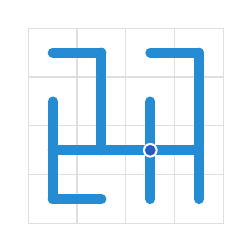
\begin{tikzpicture}[scale=.62]
\board{2,12,2,12,4,5,4,5,7,11,15,13,3,8,1,1}{water}
\end{tikzpicture}
\end{columns}
\end{frame}

\begin{frame}{Instructor and team members}
\teamfont
\textbf{Course:} Introduction to Artificial Intelligence (\CourseCode)\par\vspace{3mm}
\textbf{Instructor:} \InstructorName\par\vspace{2mm}
\textbf{Class:} \ClassName\quad$\cdot$\quad\textbf{Semester:} \Semester
\vspace{5mm}
\begin{center}
\renewcommand{\arraystretch}{1.25}
\begin{tabular}{@{}ll@{}}\toprule
\textbf{Full name} & \textbf{Student ID}\\\midrule
\StudentRows\\\bottomrule
\end{tabular}
\end{center}
\end{frame}

% Pipes frames — English version, \input from slides/main-en.tex.
% \tile/\board/\src are defined in the main-en.tex preamble.

\begin{frame}{Goal: one connected, acyclic network}
\begin{columns}[c,onlytextwidth]
\column{.38\textwidth}\centering
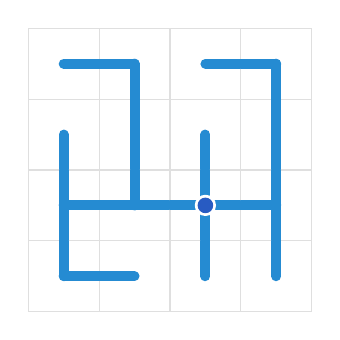
\begin{tikzpicture}[scale=.9]
\board{2,12,2,12,4,5,4,5,7,11,15,13,3,8,1,1}{water}
\end{tikzpicture}
\column{.57\textwidth}
\begin{itemize}
\item Every port matches its neighbor.
\item No port leaves the grid.
\item All tiles connect. No cycles.
\end{itemize}
\vspace{4mm}
Tiles are vertices, connections are edges.
\[
G\text{ is a tree} \quad\Longrightarrow\quad |E|=n-1
\]
\small The blue source anchors water visualization.
\end{columns}
\src{Rules: puzzle-pipes.com. Goal validation: model.py and search.py.}
\end{frame}

\begin{frame}{Problem formulation}
\small
\begin{tabular}{@{}p{.23\textwidth}p{.70\textwidth}@{}}
\toprule
Input & $n=m^2$ tiles, fixed shapes, ordinary boundaries \\
State & Prefix $s=(a_0,\ldots,a_{k-1})$ of assigned orientations \\
Initial state & Empty prefix $()$, with all tile shapes known \\
Action & Assign a rotation to tile $k$ in row-major order \\
Transition & $s'=s+(a_k)$, accepted after feasibility checks \\
Goal & $k=n$ and the complete board passes all rules \\
Cost & Unit assignment cost, unused by either ranking \\
\bottomrule
\end{tabular}\par
\vspace{5mm}
\normalsize A solver assignment can represent several manual clicks.\par
\small Any valid solution is acceptable. Minimum-click solutions are outside scope.
\src{Implemented state model: Search in pipes\_problem/search.py.}
\end{frame}

\begin{frame}{Legal successors}
The next tile has a fixed shape. Search chooses its orientation.
\vspace{5mm}
\begin{center}
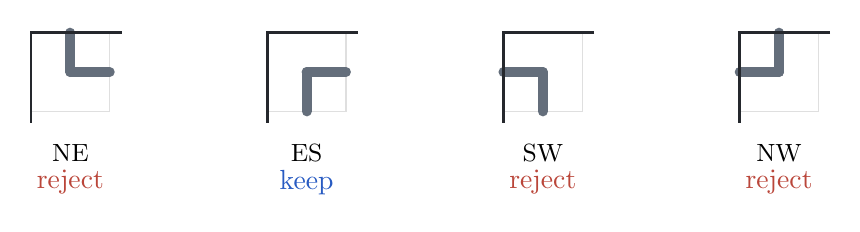
\begin{tikzpicture}[x=1cm,y=1cm]
\foreach \mask/\x/\label in {3/0/NE,6/3/ES,12/6/SW,9/9/NW}{
  \begin{scope}[shift={(\x,0)}]
    \tile{0}{0}{\mask}{muted}
    \draw[ink,line width=1pt] (.65,.5)--(-.5,.5)--(-.5,-.65);
    \node[below=8mm] at (0,0) {\small\label};
  \end{scope}}
\node[red] at (0,-1.4) {reject};
\node[blue] at (3,-1.4) {keep};
\node[red] at (6,-1.4) {reject};
\node[red] at (9,-1.4) {reject};
\end{tikzpicture}
\end{center}
\small Top-left corner example. The left and top borders forbid N and W.\par
\vspace{4mm}
\normalsize Neighbor matching also checks absent ports.\par
\small A candidate must pass every shared pruning check before search accepts it.
\src{Example is schematic. Orientation filtering: boundary\_domains() and compatible().}
\end{frame}

\begin{frame}{Search space}
\begin{columns}[T,onlytextwidth]
\column{.48\textwidth}
\small Distinct rotations per tile\par\vspace{3mm}
\begin{tabular}{@{}lr@{}}\toprule
End, elbow, T-junction & 4\\
Straight & 2\\
Cross & 1\\\bottomrule
\end{tabular}
\vspace{4mm}
\normalsize
\[U=\prod_{i=0}^{n-1}|R_i|\leq 4^n\]
\small Complete assignments before boundary checks.
\column{.47\textwidth}
\small Prefix tree\par\vspace{3mm}
\begin{tikzpicture}[every node/.style={font=\small},level distance=10mm,
 level 1/.style={sibling distance=24mm},level 2/.style={sibling distance=11mm}]
\node {$()$}
 child {node {$a_0$} child {node {$a_1$}} child {node {$a'_1$}}}
 child {node {$a'_0$} child {node {$\cdots$}}};
\end{tikzpicture}
\par\small Depth $n$, branching factor at most 4.\par
Each prefix has one parent.
\end{columns}
\vspace{4mm}
For the shipped 4\,$\times$\,4 example: $U=268{,}435{,}456$.\par
\small This bound counts assignments, not measured expansions.
\src{Count derived from distinct rotations in pipes-4x4-261.json.}
\end{frame}

\begin{frame}{Shared pruning}
\centering
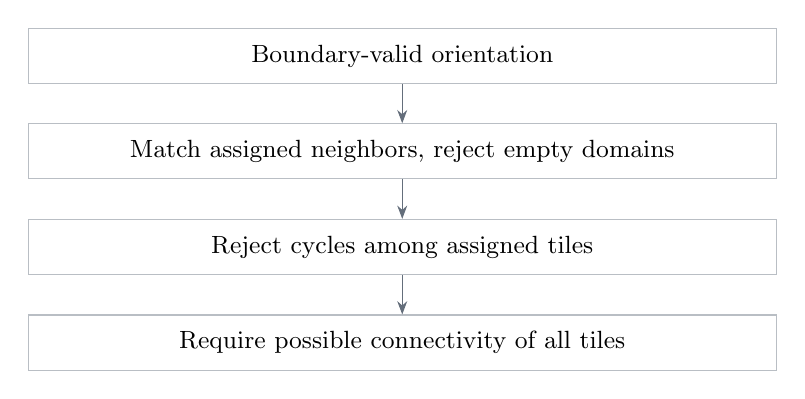
\begin{tikzpicture}[node distance=5mm,
 test/.style={draw=muted!45,minimum width=95mm,minimum height=7mm,font=\small},
 link/.style={-{Stealth},draw=muted}]
\node[test] (a) {Boundary-valid orientation};
\node[test,below=of a] (b) {Match assigned neighbors, reject empty domains};
\node[test,below=of b] (c) {Reject cycles among assigned tiles};
\node[test,below=of c] (d) {Require possible connectivity of all tiles};
\draw[link] (a)--(b);\draw[link] (b)--(c);\draw[link] (c)--(d);
\end{tikzpicture}
\vspace{3mm}\par
\small Both solvers use identical checks and fixed tile order.\par
\vspace{2mm}
Root condition: total ports $=2(n-1)$.\par
Possible connectivity is necessary but does not prove a solution exists.
\src{Pruning implementation: Search.compatible(). Full reasoning: docs/pipes-analysis.md.}
\end{frame}

\begin{frame}[fragile]{Depth-first search}
\begin{columns}[T,onlytextwidth]
\column{.60\textwidth}
\begin{lstlisting}
VISIT(s):
  if budget exhausted: return LIMIT
  count expansion
  if GOAL(s): return SOLVED(s)
  for a in rotations of tile |s|:
    child = s + (a)
    if FEASIBLE(child):
      r = VISIT(child)
      if r is SOLVED or LIMIT: return r
  return UNSOLVABLE
\end{lstlisting}
\column{.35\textwidth}
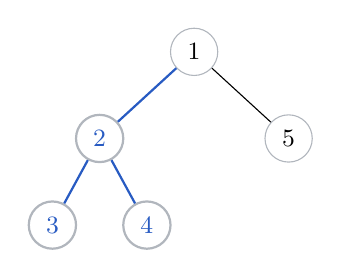
\begin{tikzpicture}[level distance=11mm,
 level 1/.style={sibling distance=24mm},level 2/.style={sibling distance=12mm},
 every node/.style={circle,draw=muted!50,minimum size=6mm,font=\small}]
\node {1}
 child[blue,thick] {node {2} child {node {3}} child {node {4}}}
 child {node {5}};
\end{tikzpicture}
\par\vspace{3mm}\small Schematic visit order.\par
Explore a branch, then backtrack.
\end{columns}
\vspace{4mm}
\small Finite-tree completeness with sufficient resources and sound pruning.\par
Worst-case exploration remains exponential.
\src{Simplified pseudocode matches dfs(). Root feasibility precedes VISIT. Cancellation is external.}
\end{frame}

\begin{frame}{Greedy's heuristic: remaining choices}
\[
h(s)=\sum_{i\text{ unassigned}}\log_2 |D_i(s)|
\]
\small $D_i(s)$ contains boundary-valid orientations matching assigned neighbors.
\vspace{5mm}
\begin{center}
\begin{tabular}{@{}lcc@{}}
\toprule
Candidate & Remaining domain sizes & $h(s)$\\\midrule
A & $(1,2,4)$ & $0+1+2=3$\\
B & $(1,1,2)$ & $0+0+1=1$\\\bottomrule
\end{tabular}
\end{center}
\vspace{3mm}
Greedy prefers B. Smaller values indicate fewer unresolved choices.\par
\small Tie order: deeper prefix, then earlier insertion.\par\vspace{3mm}
The score ignores dependencies between unassigned tiles.\par
It provides no admissibility or minimum-click guarantee.
\src{Hypothetical domain example. Exact priority: (h, -depth, insertion order) in greedy().}
\end{frame}

\begin{frame}[fragile]{Greedy Best-First search}
\begin{columns}[T,onlytextwidth]
\column{.61\textwidth}
\begin{lstlisting}
push () into min-priority queue
while queue is not empty:
  if budget exhausted: return LIMIT
  s = pop minimum-priority state
  count expansion
  if GOAL(s): return SOLVED(s)
  for a in rotations of tile |s|:
    child = s + (a)
    D = FEASIBLE(child)
    if D exists:
      push child with (h(child),
                       -|child|, serial)
return UNSOLVABLE
\end{lstlisting}
\column{.34\textwidth}
\small Queue selection\par\vspace{3mm}
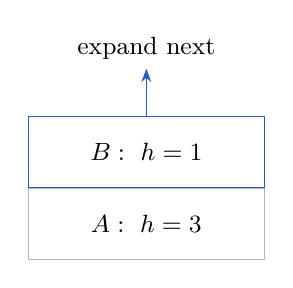
\begin{tikzpicture}[every node/.style={font=\small}]
\node[draw=blue,minimum width=30mm,minimum height=9mm] (b) {$B:\ h=1$};
\node[below=0mm of b,draw=muted!50,minimum width=30mm,minimum height=9mm] (a) {$A:\ h=3$};
\node[above=6mm of b] (pop) {expand next};
\draw[-{Stealth},blue] (b)--(pop);
\end{tikzpicture}
\par\vspace{3mm}
All feasible prefixes remain queued.\par\vspace{3mm}
Memory can grow exponentially.
\end{columns}
\src{Root feasibility precedes the queue. Priority uses h alone. The unique root starts at zero.}
\end{frame}

\begin{frame}{Evaluation protocol}
\begin{itemize}
\item Same nine saved maps for both algorithms.
\item Three maps per size, five repeats per algorithm.
\item Shared pruning, tile order and resource limits.
\end{itemize}
\vspace{4mm}
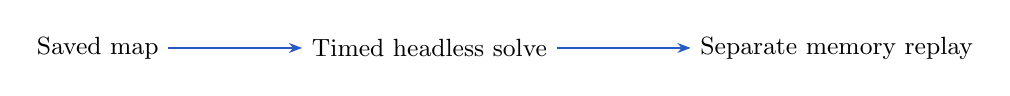
\begin{tikzpicture}[every node/.style={font=\small},node distance=17mm]
\node (map) {Saved map};
\node[right=of map] (time) {Timed headless solve};
\node[right=of time] (mem) {Separate memory replay};
\draw[-{Stealth},blue] (map)--(time);
\draw[-{Stealth},blue] (time)--(mem);
\end{tikzpicture}
\vspace{4mm}\par
\small Time excludes drawing and playback. Peak memory counts traced Python
allocations. Combine passes only when outcomes agree.\par\vspace{3mm}
Limits: 30 seconds of solver computation and 200,000 expansions.
\src{Runner: benchmark.py. Measurement: measure() and worker.py.}
\end{frame}

\begin{frame}{Baseline results}
% Source: docs/benchmarks/2026-10-25-pipes.csv, successful-run group medians (Linux, 25 Oct 2026).
\begin{center}
\small
\begin{tabular}{@{}llrrr@{}}
\toprule
Size & Algorithm & Solved/runs & Time (ms) & Peak (KiB)\\
\midrule
$4\times4$ & DFS    & 15/15 & 3.149  & 26.984\\
           & Greedy & 15/15 & 3.097  & 12.359\\
$5\times5$ & DFS    & 15/15 & 5.261  & 53.297\\
           & Greedy & 15/15 & 6.157  & 19.219\\
$7\times7$ & DFS    & 15/15 & 24.469 & 145.852\\
           & Greedy & 15/15 & 31.695 & 27.594\\
\bottomrule
\end{tabular}
\end{center}

\vspace{3mm}
\small Median over 15 successful runs per size and algorithm.\par
Each group contains three distinct inputs with five timing repeats.\par\vspace{3mm}
DFS wins at 5$\times$5 and two of three 7$\times$7 maps; Greedy takes the hardest
map (38.2 vs 40.8\,ms) and holds 4--5$\times$ less traced memory.\par
These inputs are easy under shared pruning; no general winner is claimed.
\src{Measured 25 October 2026, Linux, Python 3.13. Raw rows: docs/benchmarks/2026-10-25-pipes.csv.}
\end{frame}

\begin{frame}{Scope and next experiments}
\begin{itemize}
\item Compare harder maps and proven-unsolvable inputs.
\item Measure the effect of shared pruning separately.
\item Keep UNSOLVABLE distinct from LIMIT or CANCELLED.
\item Try alternative heuristics (MRV) and broader input sets.
\end{itemize}
\vspace{5mm}
\small\textbf{References}\par\vspace{2mm}
Pipes rules: \url{https://www.puzzle-pipes.com/}\par
Russell and Norvig, \emph{Artificial Intelligence: A Modern Approach},
4th ed., Chapters 3 and 6. \url{https://aima.cs.berkeley.edu/}
\end{frame}

% Light Up frames — English version, \input from slides/main-en.tex.

\begin{frame}{Problem 2: Light Up (Akari)}
\begin{columns}[c,onlytextwidth]
\column{.42\textwidth}\centering
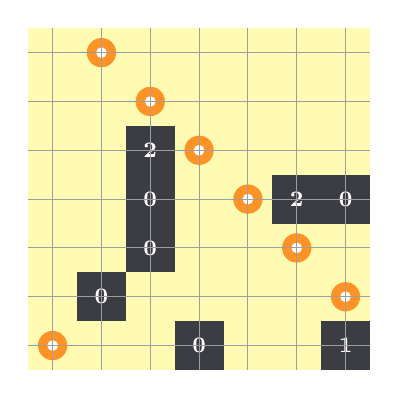
\begin{tikzpicture}[scale=.62]
  \foreach \r in {0,...,6}
    \foreach \c in {0,...,6}
      \fill[yellow!30] (\c-.5,-\r-.5) rectangle (\c+.5,-\r+.5);
  \foreach \r/\c/\v in {2/2/2,3/2/0,3/5/2,3/6/0,4/2/0,5/1/0,6/3/0,6/6/1}{
    \fill[ink!90] (\c-.5,-\r-.5) rectangle (\c+.5,-\r+.5);
    \node[white,font=\footnotesize\bfseries] at (\c,-\r) {\v};}
  \foreach \r/\c in {0/1,1/2,2/3,3/4,4/5,5/6,6/0}{
    \fill[orange!85] (\c,-\r) circle (.30);
    \fill[white] (\c,-\r) circle (.11);}
  \draw[ink!45] (-.5,.5) grid (6.5,-6.5);
\end{tikzpicture}
\column{.55\textwidth}
\begin{itemize}
\item Place bulbs on \textbf{white cells}; each bulb shines in 4 directions
until a wall or the edge.
\item Every white cell must be illuminated.
\item No two bulbs may see each other.
\item A wall numbered $k$ has exactly $k$ adjacent bulbs.
\end{itemize}
\vspace{3mm}
\small Real sample board: \texttt{akari-7-easy-70097} from the generator;\par
the picture shows its 7-bulb solution.\par
\src{Rules: puzzle-light-up.com. Board: generator/generate.py, seed 70097.}
\end{columns}
\end{frame}

\begin{frame}{Problem formulation}
\small
\begin{tabular}{@{}p{.23\textwidth}p{.70\textwidth}@{}}
\toprule
Input & Board: \texttt{None} (white), $-1$ (wall), $0..4$ (numbered wall) \\
State & Bulb set encoded as a \textbf{$W$-bit bitmask} ($W$ = white cells) \\
Initial state & Empty set (mask 0) \\
Action & Place a bulb on an eligible white cell \\
Transition & Set the bit; reject rule-breaking or unreachable successors \\
Goal & All white cells lit, all clues exact, no conflicts \\
Cost & One per placed bulb (A*'s objective) \\
\bottomrule
\end{tabular}\par
\vspace{5mm}
\normalsize Both solvers branch on the \textbf{first unlit cell (row-major)}:
only legal bulbs illuminating it are considered.\par
\small One parent per state $\Rightarrow$ no complex duplicate machinery; the
comparison between solvers stays fair.
\src{Implemented model: \_View.branch\_cell in light\_up\_problem/algorithms/search.py.}
\end{frame}

\begin{frame}{Shared sound pruning}
\centering
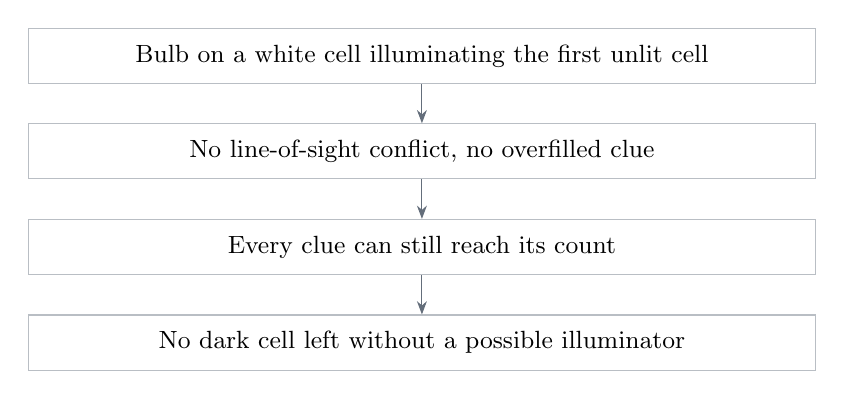
\begin{tikzpicture}[node distance=5mm,
 test/.style={draw=muted!45,minimum width=100mm,minimum height=7mm,font=\small},
 link/.style={-{Stealth},draw=muted}]
\node[test] (a) {Bulb on a white cell illuminating the first unlit cell};
\node[test,below=of a] (b) {No line-of-sight conflict, no overfilled clue};
\node[test,below=of b] (c) {Every clue can still reach its count};
\node[test,below=of c] (d) {No dark cell left without a possible illuminator};
\draw[link] (a)--(b);\draw[link] (b)--(c);\draw[link] (c)--(d);
\end{tikzpicture}
\vspace{3mm}\par
\small The checks only discard states that cannot reach a goal $\Rightarrow$
completeness preserved.\par
This is why ``blind'' DFS is fast on small and medium boards.
\src{Implementation: \_View.feasible() in algorithms/search.py.}
\end{frame}

\begin{frame}[fragile]{Blind search: Depth-First Search}
\begin{columns}[T,onlytextwidth]
\column{.60\textwidth}
\begin{lstlisting}
DFS(puzzle, limits):
  push mask 0 onto the stack
  while stack is not empty:
    if budget exhausted: return LIMIT
    state = stack.pop()
    if state in visited: continue
    if GOAL(state): return SOLVED(state)
    cell = FIRST_UNLIT_CELL(state)
    for c in bulbs illuminating cell:
      child = state | bit(c)
      if FEASIBLE(child): push child
  return UNSOLVABLE
\end{lstlisting}
\column{.36\textwidth}
\small LIFO stack + visited set.\par\vspace{3mm}
Fixed branching order,\par no heuristic information.\par\vspace{3mm}
Worst case $O(2^W)$ states.\par\vspace{3mm}
Returns the \textbf{first} solution --- not minimum-bulb.
\end{columns}
\src{Simplified pseudocode matches depth\_first\_search(). TIMEOUT/NODE\_LIMIT/MEMORY\_LIMIT stay distinct from UNSOLVABLE.}
\end{frame}

\begin{frame}{A*'s heuristic: three lower bounds, take the max}
\[
h(n)=\max\left\{\left\lceil \tfrac{D}{G_{\max}} \right\rceil,\;
\max_w d_w,\;\left\lceil \tfrac{\sum_w d_w}{H_{\max}} \right\rceil\right\}
\qquad f=g+h,\quad g=\#\text{bulbs}
\]
\small $D$: remaining dark cells; $G_{\max}$: most cells one legal bulb lights;\par
$d_w$: numbered wall $w$'s deficit; $H_{\max}$: most adjacencies one bulb satisfies.
\vspace{4mm}
\begin{center}
\begin{tabular}{@{}ll@{}}
\toprule
Component & Why it lower-bounds\\
\midrule
$\lceil D/G_{\max}\rceil$ & One bulb lights at most $G_{\max}$ dark cells\\
$\max_w d_w$ & A wall short by $d_w$ needs at least $d_w$ bulbs\\
$\lceil \sum_w d_w/H_{\max}\rceil$ & The total deficit needs that many bulbs\\
\bottomrule
\end{tabular}
\end{center}
\vspace{3mm}
Max of lower bounds is a lower bound $\Rightarrow$ $h$ is
\textbf{admissible} $\Rightarrow$ A* returns a \textbf{minimum-bulb} solution
when it completes.
\src{Implementation: \_View.lower\_bound() in algorithms/search.py.}
\end{frame}

\begin{frame}[fragile]{A* search}
\begin{columns}[T,onlytextwidth]
\column{.60\textwidth}
\begin{lstlisting}
ASTAR(puzzle, limits):
  push (f=h(0), g=0, mask 0) into min-heap
  best_g = {0: 0}
  while heap is not empty:
    if budget exhausted: return LIMIT
    pop state with minimum f
    if GOAL(state): return SOLVED(state)
    for c in bulbs illuminating
        FIRST_UNLIT_CELL(state):
      child = state | bit(c)
      if FEASIBLE(child) and
         g+1 < best_g.get(child, inf):
        best_g[child] = g+1
        push (g+1+h(child), g+1, child)
  return UNSOLVABLE
\end{lstlisting}
\column{.36\textwidth}
\small The min-heap keeps the \textbf{whole frontier}.\par\vspace{3mm}
The \texttt{best\_g} table fights rediscovery.\par\vspace{3mm}
Each expansion recomputes three bounds over large bitmasks.\par\vspace{3mm}
Memory can grow exponentially --- visible in the data.
\end{columns}
\src{Simplified pseudocode matches astar(). Unit costs make f monotone along paths.}
\end{frame}

\begin{frame}{Seeded inputs with a verified witness}
\begin{itemize}
\item Build a cyclic \emph{witness}: exactly one bulb per row and column.
\item Propose walls only where the witness survives; derive clue numbers from
adjacent witness bulbs.
\item Keep a wall only if the witness \emph{remains a valid solution} (checked
with the same \texttt{is\_goal\_state} used in play).
\end{itemize}
\vspace{4mm}
\begin{center}
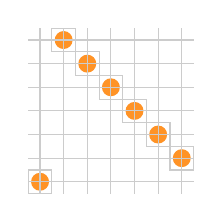
\begin{tikzpicture}[scale=.30]
  \foreach \r/\c in {0/1,1/2,2/3,3/4,4/5,5/6,6/0}{
    \draw[gray!40] (\c-.5,-\r-.5) rectangle (\c+.5,-\r+.5);
    \fill[orange!85] (\c,-\r) circle (.38);}
  \draw[gray!40] (-.5,.5) grid (6.5,-6.5);
\end{tikzpicture}
\hspace{8mm}
\begin{tabular}{@{}l@{}}
\small 4 sizes: 7, 10, 14, 25\\[1mm]
\small 3 difficulties: 16\%/10.5\%/5.5\% walls\\[1mm]
\small 12 sample sets covering all combinations\\[1mm]
\small JSON \texttt{lightup-puzzle-v1}\\[1mm]
\small \textcolor{red}{Uniqueness not checked}
\end{tabular}
\end{center}
\vspace{3mm}
\small Difficulty labels are structural (wall density), not calibrated against
solve times.
\src{Implementation: generator/generate.py. The witness is not stored in the player board.}
\end{frame}

\begin{frame}{Visual demo in pygame}
\begin{itemize}
\item \textbf{Manual play}: click to place or remove bulbs; lit cells
highlighted, conflicts outlined in red, walls show live counts.
\item \textbf{Live search}: Run / Pause / Step / Stop with expanded / generated /
frontier counters and the current bulb set (sampled events).
\item \textbf{Compare DFS and A*} on the same board: time, nodes and bulb counts
side by side.
\item \textbf{Play solution}: replay the returned placements step by step.
\end{itemize}
\vspace{4mm}
\small Solvers run in a separate spawn-safe process so the UI never stalls;\par
solver time/node/memory limits apply inside the demo too.
\src{Implementation: ui/app.py + worker.py.}
\end{frame}

\begin{frame}{Measurement protocol}
\begin{itemize}
\item 12 sample inputs: 4 sizes $\times$ 3 difficulties, 3 repeats per algorithm.
\item Limits: 30\,s, 500{,}000 nodes, 512\,MB estimated memory.
\item Same boards and limits for DFS and A*.
\end{itemize}
\vspace{4mm}

\begin{tikzpicture}[every node/.style={font=\small},node distance=24mm]
\node (map) {Seeded board};
\node[right=of map] (time) {Solver's own \texttt{perf\_counter}};
\node[right=of time] (mem) {\texttt{tracemalloc}};
\draw[-{Stealth},blue] (map)--(time);
\draw[-{Stealth},blue] (time)--(mem);
\end{tikzpicture}
\vspace{4mm}\par
\small Same machine and day as the Pipes tables (Linux, Python 3.13.14) so both
puzzles are comparable.\par
72 raw runs: \texttt{docs/benchmarks/2026-10-25-lightup.csv}.
\src{Runner: light\_up\_problem.benchmark. Evidence: docs/benchmarks/2026-10-25-lightup.md.}
\end{frame}

\begin{frame}{Results: DFS is fast and light, A* is optimal but expensive}
\small
\begin{tabular}{@{}llrrl@{}}
\toprule
Input & DFS: time / nodes & A*: time / nodes & Bulbs (DFS $\to$ A*)\\
\midrule
7 easy   & 0.026\,s / 8    & 0.273\,s / 70   & $7 = 7$\\
7 normal & 0.016\,s / 9    & 0.236\,s / 153  & $8 \to \mathbf{7}$\\
7 hard   & 0.027\,s / 7    & 6.77\,s / 3164  & $6 = 6$\\
10 easy  & 0.549\,s / 248  & 3.50\,s / 618   & $11 \to \mathbf{10}$\\
10 normal& 0.057\,s / 13   & 26.7\,s / 5464  & $12 \to \mathbf{9}$\\
10 hard  & 0.078\,s / 12   & \textcolor{red}{TIMEOUT 30\,s} (3621\,KiB) & ---\\
14 (all) & 0.35--0.42\,s / 15--17 & \textcolor{red}{TIMEOUT $\times$3} & ---\\
25 (all) & 6.7--9.7\,s / 33--35   & \textcolor{red}{TIMEOUT $\times$3} & ---\\
\bottomrule
\end{tabular}
\vspace{3mm}
\begin{itemize}
\item DFS solves \textbf{12/12} thanks to ``first unlit'' branching + pruning:
almost no backtracking (nodes $\approx$ 1.3$\times$ bulbs).
\item A* completes \textbf{5/12}, 9--250$\times$ slower, but proves optimality:
10-normal needs only 9 bulbs, not 12 (DFS overshoots 33\%).
\item Rerunning A* with a \textbf{600 s} budget: all 7 inputs still TIMEOUT
(10-hard: 151k nodes, $\sim$70 MiB) --- TIMEOUT is \emph{inconclusive}, never
unsolvable.
\end{itemize}
\src{Median of 3 runs (30 s) plus one 600 s run each, measured 25 October 2026, Linux. Data: docs/benchmarks/2026-10-25-lightup*.csv.}
\end{frame}

\begin{frame}{Limitations and next steps}
\begin{itemize}
\item Difficulty labels come from wall density, not calibrated solve times.
\item Solution uniqueness is not checked.
\item tracemalloc measures peak Python allocations, not process RSS.
\item Stronger lower bounds (matching over dark cells) could push A* further.
\end{itemize}
\vspace{5mm}
\small\textbf{References}\par\vspace{2mm}
Akari rules: \url{https://www.puzzle-light-up.com/}\par
Russell \& Norvig, \emph{Artificial Intelligence: A Modern Approach}, 4th ed.,
Chapter 3.\par
Full analysis: \texttt{docs/lightup-analysis.md}.
\end{frame}


% ---------- Closing ----------
\begin{frame}{Summary}
\begin{itemize}
\item Pipes: DFS / Greedy. Updated Light Up experiment: DFS / MRV + CP.
\item Visual demos show complete search steps; CSP also shows forced deductions.
\item New Light Up evidence: 60 distinct boards, 120 paired runs, unchanged limits.
\item Report solve rates and TIMEOUT / NODE\_LIMIT / MEMORY\_LIMIT separately.
\item Data: \texttt{docs/benchmarks/2026-10-31-lightup-dfs-csp.csv}.
\end{itemize}
\vspace{5mm}
\small\textbf{References}\par\vspace{2mm}
\url{https://www.puzzle-pipes.com/} $\cdot$ \url{https://www.puzzle-light-up.com/}\par
Russell \& Norvig, \emph{Artificial Intelligence: A Modern Approach}, 4th ed.\par
Implementation and analysis: \texttt{pipes\_problem/}, \texttt{light\_up\_problem/}, \texttt{docs/}.
\end{frame}

\end{document}
